\documentclass[main.tex]{subfiles}
\begin{document}
  \section{Evaluating the Model}
      
      The model has been assessed by comparing it to data from real matches. In this process a small subset of data was dedicated as the "training" set, and used to adjust the model and inform modelling decisions. The remaining data was designated the "test" set that was used upon development completion to evaluate the model.
      
      \subsection{Data Aquision}
        
        Data was taken from the FIVB Men's World Championship, while focusing on Poland's team, by noting down relevant data in excel. This was done early on in development and took note of all factors that were considered possibly relevant.
        \\\\
        Based on the impressions these games left it was possible to form design decisions, in particular those that fine tuned the model. For example, position 3 stands out by being extremely viable when the setter is close, but otherwise being a bad choice. In most positions a fair amount of distance is acceptable.
        
      \subsection{Analysis}
        
        The single most powerful description of the model's accuracy proved to be its ability to find the best position to set to. This should be the position that is scored highest by the model. As there is no real world data on what the setter would have considered the second best choice at the time, this is largely the only parameter available to asses the accuracy of the model.
        \\\\
        For each prediction the model records whether the real setter's choice was scored highest (i.e. 1), second highest (i.e. 2) etc,  which was dubbed the choice-rank-score. After development completed the model was tuned to maximise the choice-rank-score. \Cref{fig:training} shows the model's performance after tuning. Subsequently \Cref{fig:test} shows the choice-rank-score on the larger test set. It would appear that the larger the data set the more clearly the choice-rank-score follows some linear curve.
        \\\\
        \begin{figure}[h!]
          \begin{subfigure}{0.5\linewidth}
            \centering
            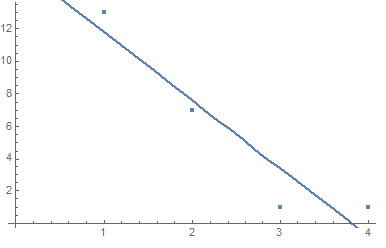
\includegraphics[width=0.70\linewidth]{figures/trainingGraph}
            \caption{Model Performance on Training Data}
            \label{fig:training}
          \end{subfigure}
          \begin{subfigure}{0.5\linewidth}
            \centering
            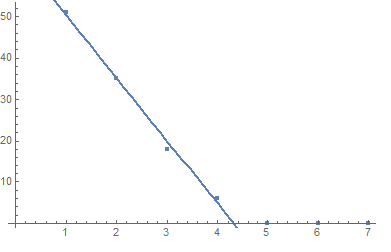
\includegraphics[width=0.70\linewidth]{figures/testGraph}
            \caption{Model Performance on Test Data}
            \label{fig:test}
          \end{subfigure}
          \caption{Model Performance on Training and Test Data Sets. \\
            Trendlines show that the model is representative of the choices made by a real setter. Null Hypotheses were rejected at the 5\% margin for training and at the 1\% margin for the test set. \\
            Note that regression was performed on the valid choices, taking into account that there are at least two invalid positions that cannot be chosen at any time.
            }
          \label{fig:analysis}
        \end{figure}
        
        Clearly, the model is capable of rather accurately predicting the probability of the setter to set to a particular position.
        
      \subsection{Drawbacks}
        
        The most evident drawback of the model is that there are a significant number of sets that are scored only second or even third. These may mostly be attributed to the fact that setters should not be too predictable, as their opponents would be able to adapt better otherwise \cite{gameTheory}. \\
        Another limitation to the model is its tuning to one particular setter, ignoring varieties in setter personality, or even player personality.\\
        Finally, at this time the model is oblivious to the opposing team, which undoubtedly plays a significant role \cite{gameTheory}.
        \\\\
        It should be noted that, while increasing the number of relevant factors would improve the ability of the model to be accurate, it also increases the difficulty of acquiring data to tune the model and evaluate it. This may prove more limiting than our ability to identify possible factors \cite[chapter 4.4]{PrinciplesOfMathematicalModeling}.

\end{document}